 \subsubsection{Hermite's Polynomials}

For another example, let's explore the Hermite polynomial. We first note that such polynomials have an integral representation given by
\begin{equation}
	\begin{split}
		H_n(x) & \deff \frac{n!}{2\pi \ii} \int_{\Gamma} z^{-n-1} \ee^{2xz-z^2} \dd z \\
		& = \frac{n!}{2\pi \ii} \int_{\Gamma} \ee^{2xz-z^2 - (n+1)\log{(z)}} \dd z
	\end{split}
\end{equation}
Where $\Gamma$ is a contour that goeas around the origin coming and going from minus infinity such as $\Gamma = \{\lambda - \ii \delta : \lambda < 0 \} \cup \{\delta \ee^{\ii \theta}: -\pi/2 < \theta < \pi/2 \} \cup \{\lambda + \ii \delta : \lambda < 0 \}$. 
\begin{figure}[H]
	\centering
	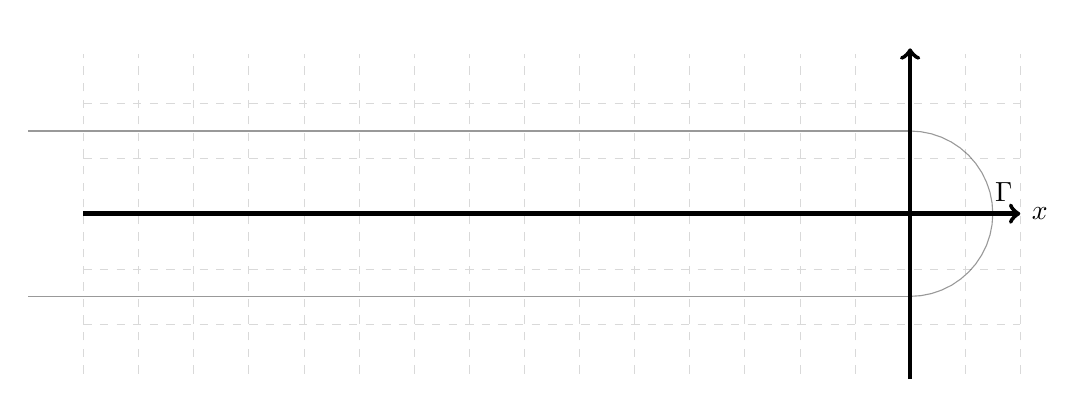
\begin{tikzpicture}[scale=.7]
		\draw[help lines, color=gray!30, dashed] (-15,-2.9) grid (2,2.9);
		\draw[->,ultra thick] (-15,0)--(2,0) node[right]{$x$};
		\draw[->,ultra thick] (0,-3)--(0,3) node[above]{$\ii$};
		
		\draw[opacity=0.4] plot[domain=-90:90] ({1.5*cos(\x)},{1.5*sin(\x)});
		\draw[opacity=0.4] plot[domain=-16:0] ({\x}, {1.5});
		\draw[opacity=0.4] plot[domain=-16:0] ({\x},{-1.5});
		
		\node (Gamma) at (1.7,0.4)    {$\Gamma$};
	\end{tikzpicture}
\end{figure}

There are a few expressions we want to have. Namely we want to determine the formulas for $H_{n}$ and  $H_{n-1}$.  Let's start working on the first case.  To do this, we only need to consider the scaling $x \mapsto N^\alpha x$ and $z = N^\beta s$ 

\begin{equation*}
	\begin{split}
		H_n(x) & = \frac{n! n^b}{2\pi \ii} \int_{\Gamma} \ee^{2(n^a \alpha)(n^b \beta)-(n^b \beta)^2 - (n+1)\log{(N^b \beta)}} \dd \beta \\
		& = \frac{n! n^b \ee^{-(n+1) \log{(n^b)}}}{2\pi \ii} \int_{\Gamma} \ee^{2(n^{a+b} \alpha \beta)-n^{2 b} \beta^2 - (n+1)\log{(\beta)}} \dd \beta \\
		& \stackrel{(a = b = 1/2)}{=}   \frac{n! \sqrt{n} \ee^{-\frac{(n+1)}{2} \log{(n)}}}{2\pi \ii} \int_{\Gamma}  \ee^{-N(-2 \alpha \beta+ \beta^2 + \log{(\beta)})} \beta^{-1} \dd \beta
	\end{split}
\end{equation*}
So that we have \[H_n(\sqrt{n}\alpha) = C_n^0 \int_{\Gamma}  \ee^{-N(\phi_\alpha(\beta))} \beta^{-1} \dd \beta\] with $\phi_\alpha(\beta) = -2 \alpha \beta+ \beta^2 + \log{(\beta)}$.  The same can be done in tehe second case, using now the reparamatrization, that is
\begin{equation*}
	\begin{split}
		H_{n-1}(x) &=  \frac{n!}{2\pi \ii} \int_{\Gamma} \ee^{2xz-z^2 - (n+1)\log{(z)}}  \\
		& = \frac{n! n^b}{2\pi \ii} \int_{\Gamma} \ee^{2(n^a \alpha)(n^b \beta)-(n^b \beta)^2 - (n+1)\log{(N^b \beta)}} \dd \beta \\
		& = \frac{n! n^b \ee^{-(n+1) \log{(n^b)}}}{2\pi \ii} \int_{\Gamma} \ee^{2(n^{a+b} \alpha \beta)-n^{2 b} \beta^2 - (n+1)\log{(\beta)}} \dd \beta \\
		& \stackrel{(a = b = 1/2)}{=}   \frac{n! \sqrt{n} \ee^{-\frac{(n+1)}{2} \log{(n)}}}{2\pi \ii} \int_{\Gamma}  \ee^{-N(-2 \alpha \beta+ \beta^2 + \log{(\beta)})} \beta^{-1} \dd \beta
	\end{split}
\end{equation*}

So that we have \[H_{n-1}(\sqrt{n}\alpha) = C_n^1 \int_{\Gamma}  \ee^{-N(\phi_\alpha(\beta))} \beta^{-\frac{1}{2}} \dd \beta\] with, again,  $\phi_\alpha(\beta) = -2 \alpha \beta+ \beta^2 + \log{(\beta)}$. As noted, for both cases, we have the same defining function $\phi_\alpha(\beta)$. As we want to calculate the asymptotic by steepest descent, we need to detemrine the critical points of such a function and then the steepest descent paths passing throught this points. We can easily determine the critical points as $\beta_c^\pm = \frac{\alpha \pm \sqrt{{\alpha}^2 - 2}}{2}$ as solutions to the quadratic formula given. Now, the behavior of the critical points will depend on the interval of the real parameter $\alpha$. We divide it into the three cases: $0 < \alpha < \sqrt{2}$, $\alpha = \sqrt{2}$ and  $\alpha > \sqrt{2}$.

\subsubsection{Case 1 }

\begin{wrapfigure}{h!}{8.5cm}
	\caption{Figure for Case 1}\label{wrap-fig:1}
	\includegraphics[width=8.5cm]{/home/vap/Documents/RMT-TEX/NotasMsC/Assets/g-contour_plot_theta_0.5.png}
\end{wrapfigure} 

Here, with $0 < \alpha < \sqrt{2}$, as the plot \ref{wrap-fig:1} suggests, we have both critical points as complex values, this can be easily determined noting that if we set $0 < \alpha < \sqrt{2}$ , we will have
\[ \beta_c^\pm  = \frac{\alpha}{2} \pm \frac{\ii}{2}\sqrt{2 -\alpha^2}.\]
And, if we parametrize $\alpha = \sqrt{2} \cos{(\gamma)}$ for $\gamma \in (0, \pi/2)$ we can rewrite 
\[ \beta_c^\pm = \frac{\sqrt{2}}{2} \ee^{\pm \ii \gamma}.\]

If we are indeed interested in solving the paths where the imaginary parts are constant, as needed for the Laplace method, we will have to sove an equation such as 
\[ \Im(\phi_{\alpha}(z) - \phi_{\alpha}(\beta_c^\pm)) = 0,\] 
for some $z = r \ee^{\ii \theta}$. We first solve for the positive critical point and he negative will be analogous. This can be rewritten as  as quadratic equation 
\[ r^2 \sin{(2\theta)} - 2r \cos{(\gamma)}\sin{(\theta)} + (\theta - \theta_0) = 0\]
where we have set $\theta_0 = \gamma - \frac{1}{2} \sin{(2\gamma)}.$ Where we solve for the two solutions $r_a^+$ and $r_d^-$  by meshing the two quadratic solutinos given by the equations. This give us two smooth paths for the positive critical point

\begin{multicols}{2}
		\begin{center}
					\includegraphics[width=6.5cm]{/home/vap/Documents/RMT-TEX/NotasMsC/Assets/geogebra-export.png}
		\end{center}
	\columnbreak
	\hspace{1cm}
	\begin{equation*}
		r_d^+(\theta)  = 
		\begin{cases}
			\frac{\sqrt{2}  \left(\cos{(\gamma)}  - \sqrt{\cos^2{(\gamma)} - (\theta - \theta_0)/(\tan{(\theta)})}  \right)}{2\cos{(\theta)}}; \ \ \theta \in [\gamma, \pi ) \\
			\frac{\sqrt{2} \left(\cos{(\gamma)}  +.\sqrt{\cos^2{(\gamma)} - (\theta - \theta_0)/(\tan{(\theta)})}  \right)}{2\cos{(\theta)}}; \ \ \theta \in (0, \gamma ) 
		\end{cases}
	\end{equation*}
	\begin{equation*}
		r_a^+(\theta) = 
		\begin{cases}
			\frac{\sqrt{2}  \left(\cos{(\gamma)}  + \sqrt{\cos^2{(\gamma)} - (\theta - \theta_0)/(\tan{(\theta)})}  \right)}{2\cos{(\theta)}};  \ \ \theta \in [\gamma, \pi/2 )\\
			\frac{\sqrt{2}  \left( \cos{(\gamma)}  - \sqrt{\cos^2{(\gamma)} - (\theta - \theta_0)/(\tan{(\theta)})}  \right)}{2\cos{(\theta)}}; \ \ \theta \in [\theta_0, \gamma )
		\end{cases}
	\end{equation*}
\end{multicols}
With which we can construct both paths of constant imaginary part 
\[\Gamma_d^+ = \{ r_d^+(\theta) \ee^{\ii \theta} : \theta \in (0, \pi) \}; \ \ \ \Gamma_a^+ = \{ r_a^+(\theta) \ee^{\ii \theta} : \theta \in (0, \pi/2) \} \]
\begin{figure}[h!]
	\centering
	\includegraphics[width=9cm]{/home/vap/Documents/RMT-TEX/NotasMsC/Assets/Hermite1positivepaths.png}
\end{figure}

Analogously, for the negative part,
\[\Gamma_d^- = \{ r_d^-(\theta) \ee^{\ii \theta} : \theta \in (0, \pi) \}; \ \ \ \Gamma_a^- = \{ r_a^-(\theta) \ee^{\ii \theta} : \theta \in (0, \pi/2) \} \]
\begin{figure}[h!]
	\centering
	\includegraphics[width=10cm]{/home/vap/Documents/RMT-TEX/NotasMsC/Assets/HermiteCompletePaths.png}
\end{figure}

Now, we only need to determine the steepest descent path. This should be easy as we know the asymptotic behaviour $\phi_\alpha(t) \asymp t^2$ for $t \rightarrow \infty$ and that  $\phi_{\alpha}(t) \asymp \ln{(t)}$ for $t \rightarrow 0$. From this, follows that $\Gamma_d^+$ and $\Gamma_d^-$ are the paths we were looking for.  We create therefore, a new path $\Gamma_x$ that connects both $\Gamma_d$ at the vertical line $x$. Then, doing $\Gamma \mapsto \Gamma_d^+ \cup \Gamma_d^- \cup \Gamma_x$ and noting that, as $x$ goes to infinity, we have
\[
	\left|  \int_{\Gamma_x} g(x) \ee^{-n\phi_\alpha(\beta)} \dd \beta  \right| \leq \max_{y \in \Gamma_x}{\left|  g(x) \ee^{-n\phi_\alpha(\beta)} \right|} \int_{\Gamma_x} |\dd \beta| \stackrel{t \rightarrow \infty}{\rightarrow} 0
\] 
where $g(t)$ can be both the inverse square root or inverse function. Therefore, we only need to consider the other two paths when considering the asymptotic.

Finally, retaking the expression for the Hermite Polynomial,
\begin{equation*}
 	\begin{split}
 		 H_n(\sqrt{2n}\cos(\gamma)) &= C_n^0 \int_{\Gamma}  \ee^{-N(\phi_\alpha(\beta))} \beta^{-1} \dd \beta  = C_n^0  \left[ \int_{\Gamma_d^-}  \ee^{-N(\phi_\alpha(\beta))} \beta^{-1} \dd \beta + \int_{\Gamma_d^+}  \ee^{-N(\phi_\alpha(\beta))} \beta^{-1} \dd \beta  \right]\\
 		 & \stackrel{(Steepest)}{=}  C_n^0  \frac{\sqrt{2\pi}}{\sqrt{2n}} \left[  \frac{\ee^{-n(\phi_\alpha(\beta_c^+))}}{\ee^{\ii \gamma/2}/2} \frac{\ee^{-\ii (\theta(\beta_c^+))}}{4 \sin{(\gamma)}} + \frac{\ee^{-n(\overline{\phi_\alpha(\beta_c^+)})}}{\ee^{-\ii \gamma/2}/2} \frac{\ee^{-\ii (\overline{\theta(\beta_c^+)})}}{4 \sin{(\gamma)}}\right] \\
 		 & =  C_n^0 \frac{\sqrt{2\pi}}{2 \sin{(\gamma)}\sqrt{2n}} \left[ \ee^{-\ii(\gamma/2 + \theta(\beta_c^+)) - n \phi_\alpha(\beta_c^+)}  + \ee^{\ii \pi} \ee^{\ii(\gamma/2 +\theta(\beta_c^+)) - n \overline{\phi_\alpha(\beta_c^+)}}  \right] \\
 		 & =  C_n^0 \frac{\sqrt{2\pi}}{2 \sin{(\gamma)}\sqrt{2n}} \left[ \ee^{-\ii(\gamma/2 + \theta(\beta_c^+)) - n (-2 \alpha \beta_c^+ + (\beta_c^+)^2 + \log{(\beta_c^+)}) }  + \ee^{\ii \pi} \ee^{\ii(\gamma/2 +\theta(\beta_c^+)) - n \overline{(-2 \alpha \beta_c^+ + (\beta_c^+)^2 + \log{(\beta_c^+)}) }}  \right]  \\
 		 & =  C_n^0 \frac{\sqrt{\pi} \ee^{-n\ln{\frac{\sqrt{2}}{2}}}}{2 \sin{(\gamma)}\sqrt{n}} \left[ \ee^{-\ii(\gamma/2 + \theta(\beta_c^+) + n \gamma) - n \ee^{\ii \gamma} (-\alpha \sqrt{2} + \frac{ \ee^{\ii \gamma}}{2}) }  -  \ee^{\ii(\gamma/2 + \theta(\beta_c^+) + n \gamma) - n \ee^{-\ii \gamma} (-\alpha \sqrt{2} + \frac{ \ee^{-\ii \gamma}}{2}) }  \right] 
 	\end{split}
\end{equation*}

Now, since
\begin{equation*}
	\begin{cases}
	Re[- n \ee^{\ii \gamma} (-\alpha \sqrt{2} + \frac{ \ee^{\ii \gamma}}{2})]= \frac{-\sqrt{2}}{2}  n; \ \ Im[- n \ee^{\ii \gamma} (-\alpha \sqrt{2} + \frac{ \ee^{\ii \gamma}}{2})] = 0 \\
	Re[ - n \ee^{-\ii \gamma} (-\alpha \sqrt{2} + \frac{ \ee^{-\ii \gamma}}{2})] = \frac{-\sqrt{2}}{2}  n; \ \  Im[ - n \ee^{-\ii \gamma} (-\alpha \sqrt{2} + \frac{ \ee^{-\ii \gamma}}{2})] = 0 .
	\end{cases}
\end{equation*}

We will have that,
\begin{equation*}
	\begin{split}
		H_n(\sqrt{2n}\cos(\gamma)) &=   C_n^0 \frac{\sqrt{\pi} \ee^{-n\ln{\frac{\sqrt{2}}{2}}}}{2 \sin{(\gamma)}\sqrt{n}} \ee^{-n \frac{\sqrt{2}}{2}} \left[ \ee^{-\ii(\gamma/2 + \theta(\beta_c^+) + n \gamma)}  -  \ee^{\ii(\gamma/2 + \theta(\beta_c^+) + n \gamma) }  \right]  \\
		&=  \frac{n! \sqrt{n} \ee^{-\frac{(n+1)}{2} \ln{(n)}}}{2\pi \ii}  \frac{\sqrt{\pi} \ee^{-n\ln{\frac{\sqrt{2}}{2}}}}{2 \sin{(\gamma)}\sqrt{n}} \ee^{-n \frac{\sqrt{2}}{2}} 2\ii \sin{\left(\gamma/2 + \theta(\beta_c^+) + n \gamma \right)} \\
		&= \frac{n!  n^{-\frac{(n+1)}{2}}}{2 \sin{(\gamma)} \pi^{\frac{3}{2}}} \ee^{-n \left( \ln{\frac{\sqrt{2}}{2}} + \frac{\sqrt{2}}{2} \right)} \sin{\left(\gamma/2 + \theta(\beta_c^+) + n \gamma \right)} 
	\end{split}
\end{equation*}

Of course, if we cange for the other case we can simply rewrite

\begin{equation*}
	\begin{split}
		H_{n-1}(\sqrt{2n}\cos(\gamma)) &=   C_n^1 \frac{\sqrt{\pi} \ee^{-n\ln{\frac{\sqrt{2}}{2}}}}{2 \sin{(\gamma)}\sqrt{n}} \ee^{-n \frac{\sqrt{2}}{2}} \left[ \ee^{-\ii(\gamma + \theta(\beta_c^+) + n \gamma)}  -  \ee^{\ii(\gamma + \theta(\beta_c^+) + n \gamma) }  \right]  \\
		&=  \frac{n! \sqrt{n} \ee^{-\frac{(n+1)}{2} \ln{(n)}}}{2\pi \ii}  \frac{\sqrt{\pi} \ee^{-n\ln{\frac{\sqrt{2}}{2}}}}{2 \sin{(\gamma)}\sqrt{n}} \ee^{-n \frac{\sqrt{2}}{2}} 2\ii \sin{\left(\gamma + \theta(\beta_c^+) + n \gamma \right)} \\
		&= \frac{n!  n^{-\frac{(n+1)}{2}}}{2 \sin{(\gamma)} \pi^{\frac{3}{2}}} \ee^{-n \left( \ln{\frac{\sqrt{2}}{2}} + \frac{\sqrt{2}}{2} \right)} \sin{\left(\gamma + \theta(\beta_c^+) + n \gamma \right)} 
	\end{split}
\end{equation*}

\subsubsection{Case 2}

\begin{wrapfigure}{h!}{8.5cm}
	\caption{Figure for case 3}\label{wrap-fig:2}
	\includegraphics[width=8.5cm]{/home/vap/Documents/RMT-TEX/NotasMsC/Assets/g-contour_plot_theta_2.png}
\end{wrapfigure} 

Here, with $ \alpha > \sqrt{2}$, as the plot \ref{wrap-fig:2} suggests, we have both critical points as real values, this can be easily determined noting that if we set $\alpha > \sqrt{2}$ , we will have
\[ \beta_c^\pm  = \frac{\alpha}{2} \pm \frac{1}{2}\sqrt{\alpha^2 - 2}.\]
And, if we parametrize $\alpha = \sqrt{2} \cosh{(\gamma)}$ for $\gamma > 0$ we can rewrite 
\[ \beta_c^\pm = \frac{\sqrt{2}}{2} \ee^{\pm \gamma}.\]

If we are indeed interested in solving the paths where the imaginary parts are constant, as needed for the Laplace method, we will have to sove an equation such as 
\[ \Im(\phi_{\alpha}(z) - \phi_{\alpha}(\beta_c^\pm)) = 0,\] 
for some $z = r \ee^{\ii \theta}$. We first solve for the positive critical point and he negative will be analogous. This can be rewritten as  as quadratic equation 
\[ r^2 \sin{(2\theta)} - 2r \cosh{(\gamma)}\sin{(\theta)} + \frac{\theta}{2} = 0\]
where we solve for the two solutions $r_a^+$ and $r_d^-$  by meshing the two quadratic solutinos given by the equations. This give us two smooth paths for the positive critical point

\begin{multicols}{2}
	\begin{center}
		\includegraphics[width=7cm]{/home/vap/Documents/RMT-TEX/NotasMsC/Assets/HermiteCase2Positive.png}
	\end{center}
	\columnbreak
	\hspace{0.2cm}
	\begin{equation*}
		r_d(\theta)  = \frac{\sqrt{2}  \left(\cosh{(\gamma)}  - \sqrt{\cosh^2{(\gamma)} - \frac{\theta}{\tan{(\theta)}} } \right)}{2\cos{(\theta)}}; \ \ \theta \in [0, \pi )
	\end{equation*}
	\begin{equation*}
		r_a(\theta)  = \frac{\sqrt{2}  \left(\cosh{(\gamma)}  + \sqrt{\cosh^2{(\gamma)} - \frac{\theta}{\tan{(\theta)}} } \right)}{2\cos{(\theta)}}; \ \ \theta \in [0, \pi )
	\end{equation*}
\end{multicols}

With which we can construct both paths of constant imaginary part 
\[\Gamma_d = \{ r_d(\theta) \ee^{\ii \theta} : \theta \in (0, \pi) \}; \ \ \ \Gamma_a = \{ r_a(\theta) \ee^{\ii \theta} : \theta \in (0, \pi) \} \]

\begin{figure}[h!]
	\centering
	\includegraphics[width=10cm]{/home/vap/Documents/RMT-TEX/NotasMsC/Assets/HermiteCase2PathsPositive.png}
\end{figure}

We need now to determine the Steepest Descent Path. In this case is more clear what the path should be the one passing through the critical point $\ee^{-\gamma}$.  Then, repeting the process we did on Case 1 - changing the path of integration - we can make the substitution
\begin{equation*}
	\begin{split}
		H_{n-1}(\sqrt{2n}\cosh{(\gamma)}) &= C_n^1 \int_{\Gamma}  \ee^{-N(\phi_\alpha(\beta))} \beta^{-\frac{1}{2}} \dd \beta \\
		&= C_n^1   \int_{\Gamma_d}  \ee^{-N(\phi_\alpha(\beta))} \beta^{-\frac{1}{2}} \dd \beta \\
		&= \stackrel{(Steepest)}{=}  C_n^1  \frac{\sqrt{2\pi}}{\sqrt{2n}} \left[  \frac{\ee^{-n(\phi_\alpha(\beta_c^+))}}{\ee^{\gamma/2}/2} \frac{\ee^{-\ii (\theta(\beta_c^+))}}{\sqrt{|1 - \ee^{2\gamma}|}}\right]  \\
		&= \frac{n! n^{-\frac{(n+1)}{2}}}{\ii  \pi^{\frac{3}{2}}} \left[  \frac{\ee^{-n(\phi_\alpha(\beta_c^+))}}{\ee^{\gamma/2}} \frac{\ee^{-\ii (\theta(\beta_c^+))}}{\sqrt{|1 - \ee^{2\gamma}|}}\right]  \\
		&= \frac{n! n^{-\frac{(n+1)}{2}}}{\pi^{\frac{3}{2}} \sqrt{|1 - \ee^{2\gamma}|} } \ee^{-n(\phi_\alpha(\beta_c^+) + \frac{\gamma}{2n})}
	\end{split}
\end{equation*}

Similary, for the other case
\begin{equation*}
	\begin{split}
		H_{n}(\sqrt{2n}\cosh{(\gamma)}) &= C_n^0 \int_{\Gamma}  \ee^{-N(\phi_\alpha(\beta))} \beta^{-1} \dd \beta \\
		&= C_n^0  \int_{\Gamma_d}  \ee^{-N(\phi_\alpha(\beta))} \beta^{-1} \dd \beta \\
		&= \stackrel{(Steepest)}{=}  C_n^1  \frac{\sqrt{2\pi}}{\sqrt{2n}} \left[  \frac{\ee^{-n(\phi_\alpha(\beta_c^+))}}{\ee^{\gamma}/2} \frac{\ee^{-\ii (\theta(\beta_c^+))}}{\sqrt{|1 - \ee^{2\gamma}|}}\right]  \\
		&=  \frac{n!n^{-\frac{(n+1)}{2}}}{\pi^{\frac{3}{2}} \ii} \left[  \frac{\ee^{-n(\phi_\alpha(\beta_c^+))}}{\ee^{\gamma}} \frac{\ee^{-\ii (\theta(\beta_c^+))}}{\sqrt{|1 - \ee^{2\gamma}|}}\right]  \\
		&= \frac{n! n^{-\frac{(n+1)}{2}}}{\pi^{\frac{3}{2}} \sqrt{|1 - \ee^{2\gamma}|} } \ee^{-n(\phi_\alpha(\beta_c^+) + \frac{\gamma}{n})}
	\end{split}
\end{equation*}



\subsubsection{Case 3}

\begin{wrapfigure}{h!}{8.5cm}
	\caption{Figure for case 3}\label{wrap-fig:3}
	\includegraphics[width=8.5cm]{/home/vap/Documents/RMT-TEX/NotasMsC/Assets/g-contour_plot_theta_1.4.png}
\end{wrapfigure} 

For the case $(1)$ we can see that the contribution for the asymptotic will come from $t_c^+$ while for case $(2)$ the contribution comes from both critical points, although depending on the real part one of the asymptotic may be exponential bigger than the other. The interesting case comes from $(3)$ where both critical point have the same value and $f''(t_c) = 0$. We need to rescale the variable somehow to get the behavior of the asymptotic. 

The idea is to perform a blow-up on the integral. We would have
$$\int_{\Gamma} \ee^{-N(-2 x t + t^2 + \log{(t)})} t^{-1} \dd t \deff \int_{\Gamma} \ee^{-N\Phi(t)} g(t) \dd t $$
where we know $\Phi$ to have first and second derivative equal to zero at $t_c = \sqrt{2}/2$. First we need to divide the integral in three parts
$$ \int_{\Gamma_1} \ee^{-N\Phi(t)} g(t) \dd t + \int_{t_c - \delta}^{t_c + \delta} \ee^{-N\Phi(t)} g(t) \dd t + \int_{\Gamma_2} \ee^{-N\Phi(t)} g(t) \dd t \approx \int_{t_c - \delta}^{t_c + \delta} \ee^{-N\Phi(t)} g(t) \dd t$$
So we would write
$$\Phi(t) = \frac{\Phi^{(3)}(t_c)}{3!} t^3 + \Boh(t^4).$$
We now want to find a change of variable $\Phi(t) = s^3$ such that $s^3 = \Phi(t) = \tilde{\Phi}(t) t^2$. If we have such an equality we know $\tilde{\Phi}$ to be analytic, $\tilde{\Phi}'(t_c) \neq 0$ and $\tilde{\Phi}(t) = \frac{\Phi^{(3)}(t_c)}{3!} t + \Boh{(  t^2)} \deff c_0 t + \Boh{(t^2)}$. 

To find such a change of variable we need to investigate the function
$$H(t, s) = t^2 \tilde{\Phi}(t) - s^3.$$
We first note that we can not find apply the Inverse Function Theorem in such a function because it's derivative is zero at $(t_c, 0)$. For that we introduce a new variable function $v = v(t)$ such that $t = v s$. Now,
$$ H(t, s) = s^3 \left( \frac{v^2}{s} \tilde{\Phi}(vs) -1 \right) \deff s^3 Q(v, s) .$$
We can of course also write $\partial_s Q(v, s) = v' \partial_v Q + \partial_s Q = 0$ giving us
$$ \frac{\partial v(t)}{\partial s} = - \frac{\partial_s Q}{\partial_v Q}.$$
It remains to check that we can indeed apply the Implicit Function Theorem to this function $Q$. For that we compute teh derivative of the function. As
$$Q(s, v(s)) = -1 + \frac{v^2}{s} (c_0 vs + \Boh(v^2s^2)) = -1 + c_0v^3 + \Boh(v^4s)$$
and because of that
$$\partial_v Q = 3 c_0 v^2 + \Boh{(v^3s)} \neq 0, \ \ \text{if} \ \ v(t_c) \neq 0.$$

Because of the theorem we can say that there exists a function $v(t)$ such that $H(vs, s) = 0$ and $v(t_c) = v_0$. Getting back to the integral we use $t = vs$ to write
\begin{equation}
	\begin{split}
		& = \int_{\alpha}^{\beta} \ee^{-Ns^3} (v(s) + v'(s)s) g(v(s)s) \dd s, \ \ \alpha = - \sqrt[3]{\Phi(\delta - t_c)} \ \ \text{and} \ \ \beta = \sqrt[3]{\Phi(\delta + t_c)} \\
		&  = \int_{\alpha}^{\beta} \ee^{-Ns^3} \frac{(v(s) + v'(s)s)}{v(s) s} \dd s \\
		& = \int_{\alpha}^{\beta} \ee^{-Ns^3} \left( \frac{1}{s} + \frac{v'(s)}{v(s)} \right) \dd s
	\end{split}
\end{equation}
where hopefully I can apply Laplace.

\begin{figure}[h] 
	\centering
	\subfigure{\includegraphics[width=0.49\textwidth]{/home/vap/Documents/RMT-TEX/NotasMsC/Assets/g-contour_plot_theta_0.png}}
	\subfigure{\includegraphics[width=0.49\textwidth]{/home/vap/Documents/RMT-TEX/NotasMsC/Assets/g-contour_plot_theta_0.5.png}}
	\subfigure{\includegraphics[width=0.49\textwidth]{/home/vap/Documents/RMT-TEX/NotasMsC/Assets/g-contour_plot_theta_1.png}}
	\subfigure{\includegraphics[width=0.49\textwidth]{/home/vap/Documents/RMT-TEX/NotasMsC/Assets/g-contour_plot_theta_1.4.png}}
	\subfigure{\includegraphics[width=0.49\textwidth]{/home/vap/Documents/RMT-TEX/NotasMsC/Assets/g-contour_plot_theta_2.png}}
	\subfigure{\includegraphics[width=0.49\textwidth]{/home/vap/Documents/RMT-TEX/NotasMsC/Assets/g-contour_plot_theta_3.png}}
	\caption{Scenarios for $x$}
	\label{Fig: x cases for hermite}
\end{figure}